%!TEX root=../GaugeCNNTheory.tex


\section{مقدمه}


\begin{figure}
	\centering
	\vspace*{-2ex}
	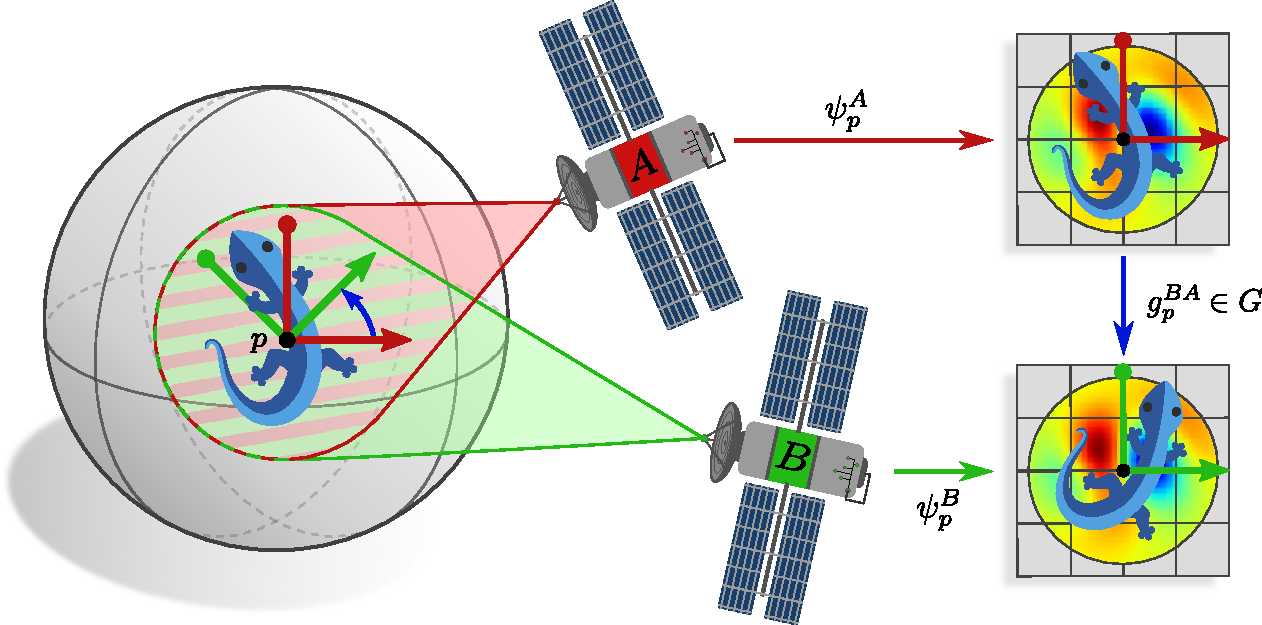
\includegraphics[width=.94\textwidth]{figures/satellite_kernels.pdf}
	\caption{\small
		ناظران مختلف A و B ممکن است یک الگوی ویژگی را از «نقطه دید» متفاوتی درک کنند.
		ماهواره‌ها در کاربرد ما، کرنل‌های کانولوشنی هستند که میدان دید محلی خود در اطراف~$p$ را در یک بردار ویژگی در~$p$ خلاصه می‌کنند.
		«نقطه دید» آن‌ها انتخابی از یک چارچوب مرجع محلی (گیج) در~p است که کرنل در امتداد آن هم‌تراز می‌شود.
		از آنجا که مشاهدات از هر دو نقطه دید یک الگوی یکسان را نشان می‌دهند، پاسخ‌های کرنل باید حاوی اطلاعات معادلی باشند، یعنی استنتاج باید \emph{مستقل از مختصات} باشد.
		این امر کرنل‌های کانولوشن را ملزم می‌کند که \emph{تحت تبدیلات گیج محلی هموردا} باشند، یعنی تغییرات چارچوب‌های مرجع.
		سطح هموردایی گیج توسط \emph{گروه ساختار}~$G$ تعیین می‌شود که هم به خمینه و هم به کاربرد بستگی دارد.
		{ \\
			\color{gray}
			\scriptsize
			(مارمولک‌ها با مجوز \href{https://github.com/twitter/twemoji/blob/gh-pages/LICENSE-GRAPHICS}{\underline{Creative Commons Attribution 4.0 International}} با تشکر از توییتر اقتباس شده‌اند.)
		}
	}
	\label{fig:satellite}
\end{figure}


در سال‌های اخیر، شبکه‌های عصبی عمیق به مدل‌های منتخب برای طیف گسترده‌ای از وظایف در یادگیری ماشین تبدیل شده‌اند.
موفقیت مدل‌های عمیق اغلب ریشه در طراحی خاص-وظیفه دارد که ساختار ریاضی داده‌های مورد پردازش را منعکس می‌کند.
یک مثال برجسته، شبکه‌های عصبی کانولوشنی (\CNN) هستند که از ساختار فضایی داده‌ها از طریق اتصال محلی و اشتراک‌گذاری وزن فضایی بهره‌برداری می‌کنند.
از آنجا که کرنل یکسانی در هر نقطه از فضا اعمال می‌شود، شبکه‌های کانولوشنی نسبت به انتقال هموردا هستند، به این معنی که الگوهای آموخته‌شده را به طور خودکار در سراسر موقعیت‌های مکانی تعمیم می‌دهند.
با توجه به موفقیت چشمگیر تجربی \CNN{}های اقلیدسی، علاقه زیادی به گسترش مدل‌های کانولوشنی برای پردازش سیگنال‌ها در دامنه‌های عمومی‌تر و هموردا ساختن آنها تحت گروه‌های تقارن بزرگ‌تر وجود دارد.


این کار به بررسی تعمیم شبکه‌های کانولوشنی به \emph{خمینه‌های ریمانی} می‌پردازد.
یک پیچیدگی عمده در تعمیم شبکه‌های کانولوشنی از فضاهای اقلیدسی $\R^d$ به خمینه‌های ریمانی عمومی این است که \emph{خمینه‌ها با انتخاب ارجحی از جهت مرجع همراه نیستند}، که بتوان یک کرنل کانولوشن را در امتداد آن برای اندازه‌گیری ویژگی‌ها هم‌تراز کرد.
از آنجا که هیچ جهت مرجعی ارجح نیست، کرنل باید به صورت \emph{دلخواه} روی خمینه هم‌تراز شود.
موضوع اصلی این کار، تنظیم این دل‌بخواهی بودن با مستقل ساختن استنتاج شبکه‌ها از هم‌ترازی خاص کرنل‌های کانولوشن است.
مشخص می‌شود که این امر نیازمند آن است که کرنل‌ها \emph{هموردای گیج} باشند، یعنی هموردا تحت تبدیلات هم‌ترازی کرنل.
پاسخ یک کرنل هموردای گیج هنگام تغییر هم‌ترازی‌اش به طور قابل پیش‌بینی تبدیل می‌شود
-- بنابراین تضمین می‌شود که محتوای اطلاعات استخراج‌شده برای هر انتخاب (دلخواه) هم‌ترازی یکسان باشد.


ما هم‌ترازی یک کرنل در نقطه‌ای~$p$ از یک خمینه $M$ را به عنوان انتخابی از یک \emph{چارچوب مرجع محلی} -- یا \emph{گیج} -- از فضای مماس متناظر $\TpM$ فرمول‌بندی می‌کنیم.
\emph{تبدیلات گیج} بنابراین تبدیلات بین انتخاب‌های چارچوب‌های مرجع هستند.
شکل~\ref{fig:intro_kernel_alignment_trivial} مفهوم هم‌تراز کردن کرنل‌ها در امتداد چارچوب‌های مرجع را به تصویر می‌کشد.
هم‌تراز کردن کرنل نسبت به \emph{میدان چارچوب} کانونی (که به طور منحصربه‌فرد ارجح است) صفحه اقلیدسی $\R^2$، همانطور که در بالا نشان داده شده، منجر به \emph{میدان کرنل} معمول \CNN{}های اقلیدسی می‌شود.
یک میدان چارچوب متفاوت، همانطور که در پایین نشان داده شده، به یک میدان کرنل جایگزین و در نتیجه یک شبکه جایگزین دلالت دارد.
همانطور که در بالا بیان شد، در بیشتر خمینه‌ها انتخاب چارچوب‌ها ذاتاً مبهم است به طوری که هیچ هم‌ترازی کرنل خاصی ارجح نیست.
شکل~\ref{fig:satellite} این موضوع را برای کره $S^2$ به تصویر می‌کشد، جایی که چارچوب‌ها تنها تا حد دوران‌ها منحصربه‌فرد هستند.


\begin{figure}[htbp]
	\centering
	% Arrange subfigures in a single row
	\begin{subfigure}[b]{0.22\textwidth}
		\centering
		
\includegraphics[width=0.8\linewidth]{figures/GpM_trivial.pdf}
		\caption{\small $G=\{e\}$}
		\label{fig:GpM_a}
	\end{subfigure}
	\hfill
	\begin{subfigure}[b]{0.22\textwidth}
		\centering
		
\includegraphics[width=0.8\linewidth]{figures/GpM_reflect.pdf}
		\caption{\small $G=\Flip$}
		\label{fig:GpM_b}
	\end{subfigure}
	\hfill
	\begin{subfigure}[b]{0.22\textwidth}
		\centering
		
\includegraphics[width=0.8\linewidth]{figures/GpM_SO2.pdf}
		\caption{\small $G=\SO2$}
		\label{fig:GpM_c}
	\end{subfigure}
	\hfill
	\begin{subfigure}[b]{0.22\textwidth}
		\centering
		
\includegraphics[width=0.8\linewidth]{figures/GpM_scale.pdf}
		\caption{\small $G=\Scale$}
		\label{fig:GpM_d}
	\end{subfigure}
	
	% Standard caption
	\caption{\small
		انتخاب چارچوب‌های مرجع یک فضای مماس $\TpM$ همیشه منحصربه‌فرد نیست.
		ساختار هندسی (ساختار $G$) یک خمینه، زیرمجموعه‌ای ارجح از چارچوب‌های مرجع را ایجاب می‌کند به طوری که تبدیلات گیج بین این چارچوب‌ها در گروه ساختار~$G\leq\GL{d}$ قرار می‌گیرند.
		شکل‌های~\ref{fig:GpM_a}، \ref{fig:GpM_b}، \ref{fig:GpM_c} و~\ref{fig:GpM_d}
		چنین زیرمجموعه‌هایی از چارچوب‌ها را به ترتیب برای گروه بدیهی $G=\{e\}$، گروه بازتاب $G=\Flip$، گروه دوران $G=\SO2$ و گروه مقیاس‌پذیری~$G=\Scale$ نشان می‌دهند.
		ویژگی‌ها اندازه‌گیری‌ها را نسبت به هر یک از چارچوب‌های متمایز کدگذاری می‌کنند.
		ضرایب عددی آن‌ها نسبت به چارچوب‌های مختلف، توسط عمل یک نمایش گروهی $\rho$ از~$G$ به هم مرتبط می‌شوند.
	}
	\label{fig:GpM_examples}
\end{figure}


سطح ابهام در انتخاب چارچوب‌های مرجع به \emph{ساختار هندسی} خمینه بستگی دارد.
چنین ساختاری اغلب امکان
\emph{رفع ابهام چارچوب‌های مرجع تا حد تبدیلات تقارنی معین} (تبدیلات گیج) را فراهم می‌کند؛ به شکل~\ref{fig:GpM_examples} مراجعه کنید.
این بیانیه با چند مثال بهتر توضیح داده می‌شود:
\begin{itemize}[leftmargin=1.2cm]
	\item[{\rule[2.2pt]{2pt}{2pt}}]
	یک \emph{خمینه هموار} خام هیچ ترجیحی در انتخاب چارچوب‌ها ندارد.
	تبدیلات گیج بین چارچوب‌های عمومی، نگاشت‌های خطی معکوس‌پذیر دلخواه هستند، یعنی مقادیری در \emph{گروه خطی عمومی} ${G=\GL{d}}$ می‌گیرند.
	\item[{\rule[2.2pt]{2pt}{2pt}}]
	یک \emph{جهت‌گیری} از خمینه امکان تمایز چارچوب‌های چپ‌گرد از راست‌گرد را فراهم می‌کند.
	تبدیلات گیج بین چارچوب‌های هر یک از دو دست، حافظ جهت‌گیری هستند، یعنی عناصری از ${G=\operatorname{GL}^+(d)}$ هستند (نگاشت‌های خطی معکوس‌پذیر با دترمینان مثبت).
	\item[{\rule[2.2pt]{2pt}{2pt}}]
	یک \emph{فرم حجم} امکان تمایز \emph{چارچوب‌های با حجم واحد} را فراهم می‌کند.
	در این صورت، تبدیلات گیج حافظ حجم هستند، یعنی مقادیری در \emph{گروه خطی ویژه} $G=\operatorname{SL}(d)$ می‌گیرند.
	\item[{\rule[2.2pt]{2pt}{2pt}}]
	\emph{ساختار متریک} یک خمینه ریمانی امکان اندازه‌گیری فواصل و زوایا را در فضاهای مماس فراهم می‌کند و بنابراین امکان تمایز \emph{چارچوب‌های متعامد} را می‌دهد.
	تبدیلات گیج بین چارچوب‌های متعامد، دوران‌ها و بازتاب‌ها در \emph{گروه متعامد} $G=\O{d}$ هستند.
	\item[{\rule[2.2pt]{2pt}{2pt}}]
	با هم، یک \emph{جهت‌گیری و متریک} به \emph{چارچوب‌های متعامد جهت‌دار} دلالت دارند.
	در این صورت، تبدیلات گیج فقط دوران‌ها در \emph{گروه متعامد ویژه} $G=\SO{d}$ هستند.
	\item[{\rule[2.2pt]{2pt}{2pt}}]
	یک \emph{میدان چارچوب} روی خمینه شامل یک \emph{چارچوب منحصربه‌فرد} در هر نقطه از خمینه است.
	در این حالت، تبدیلات گیج بدیهی هستند که توسط \emph{گروه بدیهی} $G=\{e\}$ توصیف می‌شوند.
\end{itemize}
همه این ساختارهای هندسی مشترکاً یک زیرمجموعه ارجح (زیربندل) از چارچوب‌ها را تعریف می‌کنند به طوری که تبدیلات گیج مقادیری در یک \emph{گروه ساختار}~$G\leq\GL{d}$ می‌گیرند.
برای تأکید بر نقش محوری گروه ساختار $G$، چنین ساختارهایی به عنوان $G$-\emph{ساختار}~$\GM$ نامیده می‌شوند.
مثال‌های بصری از $G$-ساختارها برای گروه‌های ساختار $G$ و خمینه‌های~$M$ مختلف در شکل~\ref{fig:G_structures_intro} آورده شده است.


از آنجا که انتخاب چارچوب‌های مرجع ذاتاً مبهم است، هر کمیت هندسی و عملیات شبکه باید به طور مساوی نسبت به چارچوب‌های دلخواه $G$-ساختار~$\GM$ قابل نمایش باشد، یعنی باید $\GM$-\emph{مستقل از مختصات} باشد.
بردارهای ویژگی بنابراین با یک \emph{نمایش گروهی} (عمل گروهی خطی) $\rho$ از گروه ساختار $G$ مرتبط هستند که قانون تبدیل آنها را تحت تبدیلات گیج (گذار‌های با مقدار $G$ بین چارچوب‌های مرجع) تعیین می‌کند.
انتخاب خاص نمایش گروهی، نوع هندسی یک میدان بردار ویژگی را تعیین می‌کند.
مثال‌های معمول شامل میدان‌های اسکالر، بردار یا تانسور هستند، با این حال، انواع میدان عمومی‌تری نیز در عمل استفاده می‌شوند.
شکل~\ref{fig:gauge_trafos} استقلال از مختصات کمیت‌های هندسی را در مثال شناخته‌شده بردارهای مماس به تصویر می‌کشد.


هر لایه شبکه ملزم به رعایت قوانین تبدیل ویژگی‌هاست، یعنی باید تضمین کند که خروجی‌هایش همانطور که انتظار می‌رود تبدیل می‌شوند.
به طور خاص برای کانولوشن‌ها، استقلال از مختصات $\GM$ ایجاب می‌کند که اعمال کرنل مشترک نسبت به چارچوب‌های مختلف $G$-ساختار در یک نقطه $p\in M$ باید \emph{پاسخ یکسانی را تا حد یک تبدیل گیج} برانگیزد.
ما نشان می‌دهیم که این امر نیازمند $G$-راهبری (هموردایی گیج، معادله~\eqref{eq:G-steerable_kernel_space}) کرنل‌های کانولوشن است.
به طور شهودی، می‌توان کرنل‌های $G$-راهبر را به عنوان اندازه‌گیری ویژگی‌ها به صورت \emph{نسبی} نسبت به چارچوب‌های مرجع تصور کرد، که این امر ضروری است زیرا هیچ انتخاب چارچوب، یعنی هم‌ترازی کرنل \emph{مطلق}، ارجح نیست.%
\footnote{
	به شباهت با \emph{اصل نسبیت خاص} انیشتین توجه کنید، که به جای چارچوب‌های $G$-ساختار، بر برابری چارچوب‌های لخت تکیه دارد.
}
مثال‌هایی از کرنل‌های $G$-راهبر برای گروه بازتاب $G=\Flip$ در شکل~\ref{fig:intro_steerable_kernel} نشان داده شده است.
شکل~\ref{fig:intro_kernel_alignment_reflect} اشتراک‌گذاری چنین کرنل‌هایی را نسبت به چارچوب‌های مختلف یک ساختار $\Flip$ به تصویر می‌کشد.
قید $\Flip$-راهبری نوعی تقارن را بر کرنل‌ها تحمیل می‌کند، به طوری که هم‌ترازی‌های مختلف واقعاً منجر به پاسخ‌هایی می‌شوند که دقیقاً با تبدیلات گیج $\rho(g)$ متفاوت هستند.
ما در ادامه کانولوشن‌های مستقل از مختصات $\GM$ را به عنوان \emph{کانولوشن‌های} $\GM$ مخفف می‌کنیم.


علاوه بر اعمال کرنل‌های \emph{هموردای گیج}، کانولوشن‌های $\GM$ ممکن است \emph{هموردای ایزومتری} باشند، به این معنی که با عمل ایزومتری‌ها بر روی میدان‌های ویژگی جابجا می‌شوند، همانطور که در شکل~\ref{fig:lizard_conv_egg_intro} نشان داده شده است.
فرض کنید $\phi \in \IsomM$ یک ایزومتری (تقارن) از خمینه~$M$ باشد.
یک شبکه عصبی دقیقاً زمانی نسبت به عمل این ایزومتری هموردا است که الگوها در هر نقطه $p\in M$ به همان روشی پردازش شوند که الگوها در~$\phi(p)$ پردازش می‌شوند.
بنابراین هموردایی ایزومتری یک شبکه در تناظر یک به یک با \emph{ناوردایی ایزومتری اتصال عصبی آن} (میدان کرنل) است؛ به شکل~\ref{fig:isom_invariant_kernel_field_intro} مراجعه کنید.
از آنجا که کانولوشن‌های ما کرنل‌ها را نسبت به چارچوب‌های (دلخواه) $G$-ساختار $\GM$ اعمال می‌کنند، تقارن‌های میدان کرنل با تقارن‌های $G$-ساختار منطبق هستند.
با نشان دادن \emph{تقارن‌های (حافظ فاصله) یک $G$-ساختار} $\GM$ با $\IsomGM \leq \IsomM$، این دلالت دارد که کانولوشن‌های ما دقیقاً $\IsomGM$-هموردا هستند.
شکل~\ref{fig:intro_invariant_kernel_fields_plane} این واقعیت را که $G$-ساختارها و میدان‌های کرنل متناظر تقارن‌های یکسانی دارند، به تصویر می‌کشد.
خواننده تشویق می‌شود که $G$-ساختارها را در شکل~\ref{fig:G_structures_intro} با توجه به تقارن‌هایشان و ویژگی‌های هموردایی ضمنی کانولوشن‌های $\GM$ متناظر بررسی کند.


طراحی شبکه‌های کانولوشنی مستقل از مختصات $\GM$ بر روی خمینه‌های ریمانی نیازمند انتخاب یک $G$-ساختار است که به ملاحظات متعددی بستگی دارد.
اولاً، انتخاب گروه ساختار~$G$ \emph{هموردایی گیج محلی} کانولوشن را تعیین می‌کند:
یک کرنل $G$-راهبر به طور خودکار الگوهای آموخته‌شده را بر روی تمام ژست‌های مرتبط با $G$ از الگوها تعمیم می‌دهد؛ به شکل~\ref{fig:intro_lizard} مراجعه کنید.
ثانیاً، انتخاب خاص $G$-ساختار \emph{هموردایی ایزومتری سراسری} کانولوشن را تعیین می‌کند.
در کاربردهای تصویربرداری پزشکی، الگوها اغلب در دوران‌ها، بازتاب‌ها و موقعیت‌های دلخواه رخ می‌دهند
-- بنابراین باید یک ساختار $\O{d}$ ناوردای $\IsomGM = \E{d}$ را روی $\R^d$ انتخاب کرد، مشابه ساختار $\SO2$ که در شکل~\ref{fig:G_structure_intro_g} نشان داده شده است.
تصاویری مانند عکس‌های پرتره یک محور عمودی متمایز دارند، با این حال، بازتاب‌ها حول این محور آمار تصویر را ناوردا می‌گذارند
-- این امر نیازمند یک ساختار $\Flip$ مانند شکل~\ref{fig:G_structure_intro_d} است.
علاوه بر چنین ملاحظات تقارنی، توجه به این نکته مهم است که هر خمینه‌ای (توپولوژی) ساختارهای $G$ \emph{هموار} را برای هر انتخاب گروه ساختار~$G$ نمی‌پذیرد.
یک مثال نوار موبیوس است که توپولوژی پیچ‌خورده آن (عدم جهت‌گیری) مانع از تخصیص هموار متغیر جهت‌گیری‌های چارچوب می‌شود.
بنابراین یک عملیات کانولوشن مستقل از مختصات \emph{هموار} بر روی نوار موبیوس \emph{لزوماً} بر کرنل‌های راهبر-بازتابی تکیه دارد.


این کار شامل یک \emph{مرور ادبیات} گسترده بر روی شبکه‌های کانولوشنی است که عمومیت نظریه ما را نشان می‌دهد.
این بخش انواع مختلفی از \CNN{}ها را در فضاهای اقلیدسی، \CNN{}های کروی و کانولوشن‌ها را بر روی سطوح عمومی (مانند مش‌های سطحی) پوشش می‌دهد.
ما انتخاب‌های خاص $G$-ساختارها را که به طور ضمنی توسط نویسندگان انجام شده است، با تحلیل ویژگی‌های هموردایی سراسری و محلی مدل‌هایشان شناسایی می‌کنیم.
جدول~\ref{tab:network_instantiations} یک نمای کلی از طبقه‌بندی حاصل از شبکه‌های کانولوشنی مستقل از مختصات $\GM$ ارائه می‌دهد.


برای ارائه یک مثال دقیق در مورد چگونگی نمونه‌سازی نظریه ما در عمل، ما پیاده‌سازی کانولوشن‌های $\GM$ را بر روی نوار موبیوس برای~$G=\Flip$ مورد بحث قرار می‌دهیم.
این شامل استخراج کرنل‌های راهبر-بازتابی برای انواع میدان مختلف (نمایش‌های گروهی) و ارزیابی تجربی هموردایی ایزومتری پیش‌بینی‌شده نظری است.
همانطور که انتظار می‌رود، کانولوشن‌های مستقل از مختصات $\GM$ از پیاده‌سازی وابسته به مختصات ساده بهتر عمل می‌کنند.
کد در آدرس \url{https://github.com/mauriceweiler/MobiusCNNs} موجود است.

یک فرمول‌بندی \emph{بدون مختصات} از نظریه ما در زبان \emph{بندل‌های فیبر} ابداع شده است.
$G$-ساختارها $\GM$ زیربندل‌های اصلی $G$ از بندل چارچوب $\FM$ بر روی~$M$ هستند.
میدان‌های ویژگی \emph{برش‌هایی} از \emph{بندل‌های بردار ویژگی مرتبط} با $G$ هستند.
گیج‌ها \emph{تسهیم‌های بندل محلی} هستند، در حالی که تبدیلات گیج نگاشت‌های گذار بین چنین تسهیم‌هایی هستند.
ایزومتری‌هایی که یک کانولوشن $\GM$ نسبت به آنها هموردا است، \emph{اتومورفیسم‌های بندل اصلی} از $G$-ساختار هستند.


\CNN{}های مستقل از مختصات ما تعمیم‌هایی از \emph{\CNN{}های راهبر}~\cite{Cohen2017-STEER,3d_steerableCNNs,Weiler2019_E2CNN,Cohen2019-generaltheory,lang2020WignerEckart} از فضاهای اقلیدسی (یا همگن) به خمینه‌های ریمانی هستند.
در حالی که \CNN{}های راهبر بر تبدیلات \emph{فعال و سراسری} میدان‌های ویژگی تمرکز دارند، \CNN{}های مستقل از مختصات تبدیلات \emph{غیرفعال و محلی} بین چارچوب‌های مرجع را در نظر می‌گیرند.%
\footnote{
	این شبیه به تغییر تمرکز از \emph{کوواریانس لورنتس سراسری} در \emph{نسبیت خاص} به \emph{کوواریانس لورنتس محلی} در \emph{نسبیت عام} است.
}
ما نسخه‌های اولیه‌ای از نظریه \CNN{}های مستقل از مختصات ("\CNN{}های هموردای گیج") را در کارهای قبلی~\cite{gaugeIco2019,deHaan2020meshCNNs} پیشنهاد کردیم.
برخلاف این انتشارات، کار حاضر نظریه را با جزئیات بسیار بیشتری توسعه می‌دهد، آن را بر حسب بندل‌های فیبر فرمول‌بندی می‌کند، هموردایی تحت عمل ایزومتری‌ها را اثبات می‌کند و یک مرور ادبیات ارائه می‌دهد.